\section{Reservoir Computing}
\label{sec:reservoir_computing}

From the description of the available training methods of RNNs in
Section~\ref{sub:training_recurrent_neural_networks}, one can see that despite
their theoretical capabilities it becomes very difficult to train them in
practice:
\begin{enumerate}
  \item Sequences that require long-range memory are almost impossible to learn,
    due to the vanishing gradient problem of BPTT based optimizers.
  \item The computational complexity of RNN training is very high, with BPTT
    having a complexity of O(n$^2$) per weight update per time step for a
    single output and even O(n$^4$) for RTRL.
  \item Bifurcations in the error surface can prevent the network from
    converging at all.
\end{enumerate}

A recent approach termed \emph{reservoir computing} (RC) that was introduced by
[\cite{lukosevicius}] promises to eliminate almost all the previous
disadvantages by making a conceptual separation between the actual RNN and the
subsequent output layer that maps its internal state to the desired output.
The recurrent part of RNN is regarded as a reservoir, which remains untrained
and only takes the role of mapping the input into a higher dimensional,
temporal representation.  A linear output layer is the only part of the network
that is optimized to produce the desired output from the internal state of the
RNN.

\subsection{Pattern Recognition in a Bucket}%
\label{sub:pattern_recognition_in_a_bucket}

The separation of the recurrent part of the RNN and the output layer is
intuitively described by an experiment called \emph{Pattern recognition in a
bucket} [\cite{Fernando2003PatternRI}], which basically substitutes the RNN with
a bucket of water.  A loudspeaker excites waves on the water surface, which is
filmed and fed into a simple, one-layer feedforward network, equivalent to the
output layer of an RNN.  The output layer is trained on the patterns that arise
from the audio input and a second control network directly on the audio signal.
The control network could not achieve error rates in the classification of
simple words below 25\%, while the networks trained on the water patters made
no more mistakes than 1.5\%.  The reason for this considerable increase in
accuracy is that the water patterns create a high dimensional representation of
the input data.  This representation does not only hold information of the
current time frame, but serves as a memory, as the disturbances in the water
propagate over the whole surface.  Most importantly, this representation is
generated by the underlying physics, which cannot be adjusted to the input
data.  The water has not undergone any kind of training, however, one can still
train the output layer on the deterministically created patterns of its
surface, which nicely illustrates the philosophy of reservoir computing.  The
recurrent weight matrices can, if appropriately initialized, give rise to
similar deterministic patterns in the internal state.


\subsection{The Echo State Network}%
\label{sub:the_echo_state_network}

\begin{figure}
  \centering
  \ESNFlowChart
  \caption{Flow chart of an echo state network. The hatched squares mark the
    untrained weight matrices.}
  \label{fig:esn_flow_chart}
\end{figure}

Mathematically, the part of the static reservoir is taken by the state-space
equation (Eq.~\ref{eq:state_space}) that was introduced in
Sec.~\ref{ssub:state_space_model}.  The weight matrices are initialized during
the setup of the network and are kept static for all times.  Only the weights
of the output layer (Eq.~\ref{eq:readout}) are optimized during the training
phase of the network. This kind of RC network, that is very close to the common
RNN is called \emph{Echo State Network} (ESN). Another kind of RC network is
the \emph{Liquid State Machine}~[\cite{maass2004}], which is studied in
computational neuroscience, as it tries to mimic the spiking neurons of the
brain. It is typically only used for research purposes as its computational
complexity is much higher because it has to compute spiking state activations
in every neuron.

Even though the reservoir is not optimized at all, it still takes the role of a
non-linear expansion into a higher dimensional space and serves as the
short-term memory of the input (Sec.~\ref{sub:short_term_memory}).  This is
possible without adjusting the recurrent weights, given that the initialization
of ESN is done carefully.  In the following we will explore the demands that
need to be made to the reservoir weights in order to ensure its functionality
as a temporal memory, which enables predictions of the future based on the past
inputs.  Assuming that the output layer alone is able to extract the desired
prediction from the current internal state, the ESN should be able to perform
the same tasks as the general RNN. Additionally the problem of bifurcations in
the error surface is eliminated, as the recurrent weights are not altered
during the training. A practical comparison between RNNs and ESNs is hard to do
and no general, objective favorite with regard to performance has been found
yet.


\subsection{The Echo State Property}
\label{sub:echo_state_property}

As the goal of the ESN is to make predictions based on the history of a given
time series, we have to construct an internal state that is a function of the
previously seen inputs, such that
\begin{equation}
  \label{eq:echo_func}
  \vt{x} = f(..., \vec{u}_{t-1}, \vt{u})
\end{equation}
without adjusting the internal weights of the network during training.
An RNN that exhibits this behaviour is said to satisfy the \emph{echo state
property} and called an ESN.  The simplest ESN provides some insight into the
temporal evolution of the internal state. It consists only of one hidden weight
matrix and does not have any external inputs:
\begin{equation}
    \label{eq:state_space_hidden_only}
    \vt{x} = \varphi(\wmatr{} \vec{x}_{t-1})
\end{equation}
By randomly initializing $\wmatr{}$, the only hyper-parameter of the ESN is the
spectral radius $\rho(\wmatr{})$, which is defined as its the largest
eigenvalue:
\begin{equation}
  \rho(\wmatr{}) = \text{max} \{|\lambda_1|, |\lambda_2|, ..., |\lambda_n|\}.
\end{equation}
There exist various libraries that efficiently calculate extremal eigenvalues
for example based on simple power methods (described
in~\ref{sec:spectral_radius}) or more sophisticated methods such as the Lanczos
algorithm~[\cite{lanczos1950iteration}].  Note that the spectral radius scales
with a factor $\alpha$:
\begin{equation}
  \label{eq:spr_scale}
  \rho(\alpha \wmatr{}) = \alpha \rho(\wmatr{}).
\end{equation}
The desired $\rho(\wmatr{})$ can therefore be easily adjusted to an arbitrary
value by multiplying with an appropriate factor.


\begin{figure}
  \centering
  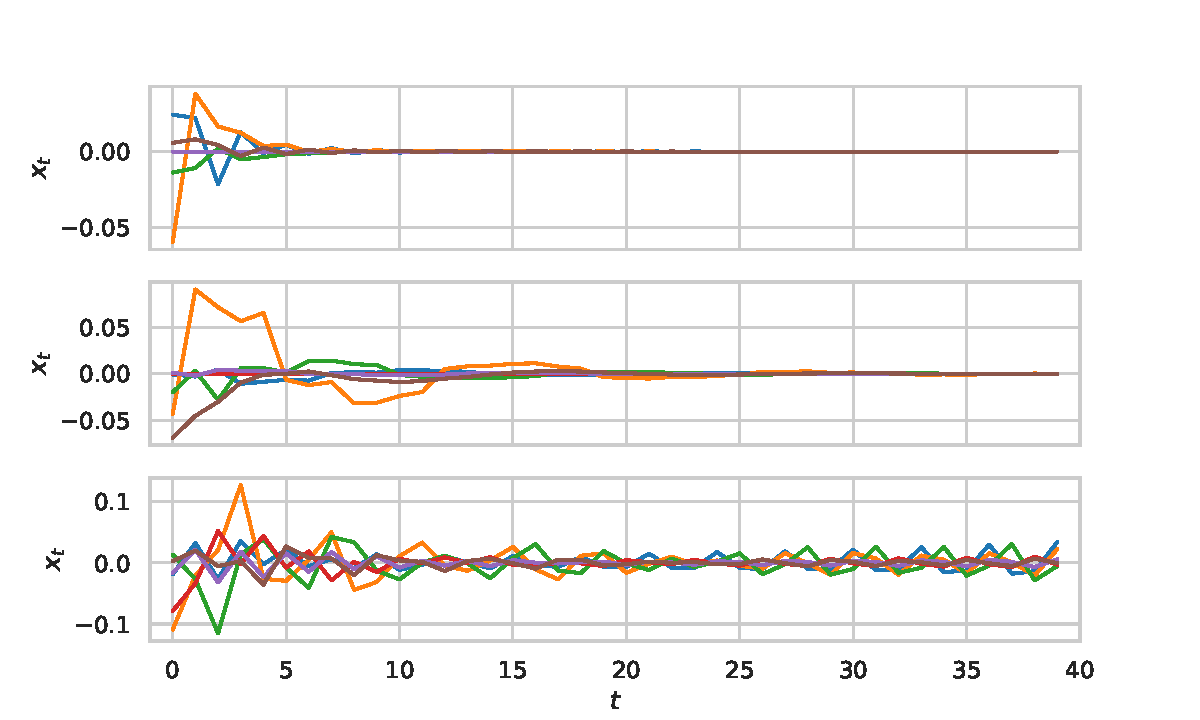
\includegraphics[width=\linewidth]{esn_states_noinput.pdf}
  \caption{State activations of the simple ESN without input weights as defined in
  Eq.~\ref{eq:state_space_hidden_only}. Each line depicts the temporal
  evolution of a single internal state unit. The initial state decays faster in
  the top graph, where the spectral radius is $\rho=0.75$, slower in the middle
  with $\rho=0.95$ and echoes indefinitely in the bottom graph with
  $\rho=1.05$.  The state dynamics are just as expected from the analysis in
  Sec.~\ref{sub:the_bifurcating_state_space}.
  }
  \label{fig:esn_states_noinput}
\end{figure}

As an example we create an initial state $x_0$ randomly from a normal
distribution and the activation function $\varphi$ is taken to be the
hyperbolic tangent.  The smaller the spectral radius, the faster the
information of the initial state should decay as the network is stepping
through time according to Eq.~\ref{eq:state_space_hidden_only}.  The two upper
plots of Fig.~\ref{fig:esn_states_noinput} show exactly this effect.  The first
plot is created by a network with $\rho=0.75$, while the second one is the
result of $\rho=0.95$. The information of the random, initial state
\emph{echoes} much longer with the larger spectral radius and as a result, the
memory of the network becomes longer.  In both cases the echo state property is
satisfied.  In [\cite{jaeger2001}] one can find the formal proof of the
sufficient condition for echo states:
\begin{equation}
  \rho(\wmatr{}) < 1,
\end{equation}
which holds for all monotonically increasing $\varphi$.  In the bottom plot of
Fig.~\ref{fig:esn_states_noinput}, one can see the effect of $\rho=1.05>1$.
Spectral radii $\rho > 1$ would, over time, lead to an exponential growth of
the state activations, if it was not for the bounded, non-linear activation
function $\varphi = \tanh(x)$.  The hyperbolic tangent prevents this divergence
and additionally, the internal state activations never settle down and will go
on echoing forever.  This strongly resembles the periodic fixed points
discussed in Sec.~\ref{sub:the_bifurcating_state_space} and has interesting,
both positive and negative implications for the networks ability to memorize
input and model predictions. Non-linear activation functions such as the
hyperbolic tangent often prevent the state from exploding, thus making it
possible to use spectral radii larger than one. This can still yield valid echo
states, but the risk of over-saturating the state becomes much higher.  This
saturation is caused by the internal dynamic that is introduced to the state by
entering the non-linear regime of the activation function and the resulting
periodic fixed points.  If the internal dynamic starts dominating the input to
the ESN it becomes useless, as all the external information is overwritten by
its internal dynamics.  The implications that a varying spectral radius has for
the performance of the ESN on different datasets is discussed in
Chapter~\ref{cha:results}.\\


\subsection{Reservoir With Inputs}
\label{sub:reservoir_without_feedback_weights}

In the more practical case of an ESN with external inputs, the internal state
and thus the memory of the network is also influenced by the degree of which
the input overwrites the previous internal state.  To incorporate a scalar
input in the network we introduce an input weight matrix $\wmatr{in}$ with
dimensions $(N \times 1)$.
\begin{equation}
  \label{eq:state_space_no_feedback}
  \vt{x} = \varphi(\wmatr{in}  \vt{u} + \wmatr{hidden} \vec{x}_{t-1}).
\end{equation}

The range of values that $\wmatr{in}$ is initialized with is a typical
hyper-parameter for which there are no solid guidelines, apart from choosing
small values.  We will choose a uniform distribution of values between $-\kappa
< 0 < \kappa$, where $\kappa$ is typically smaller than one half. The
implications of different initializations are shown in
Fig.~\ref{fig:esn_states_input}.  It shows how the internal state reacts to a
scalar input in form of a simple step function. 

For a small $\rho=0.5$ and large $\kappa=0.1$, the state $x$ is dominated by
the input, which is visualized in Fig.~\ref{fig:esn_states_input} B.  The state
activations quickly approach certain value and form a plateau after just three
to four time steps. When such a plateau is reached in all state activations,
the network cannot determine the current position in the time series any more
and will loose its predictive power.  In plot C the network is set up with
$\rho=0.9$ and $\kappa=0.02$.  It takes longer for the initial random state to
decay and the individual activations are not reaching a plateau any more.  From
the recurring state activations that are the same after each period but
different for each point within one period, the network can infer where in the
time series it currently is and make an accurate prediction for the next step.
\begin{figure}
  \centering
  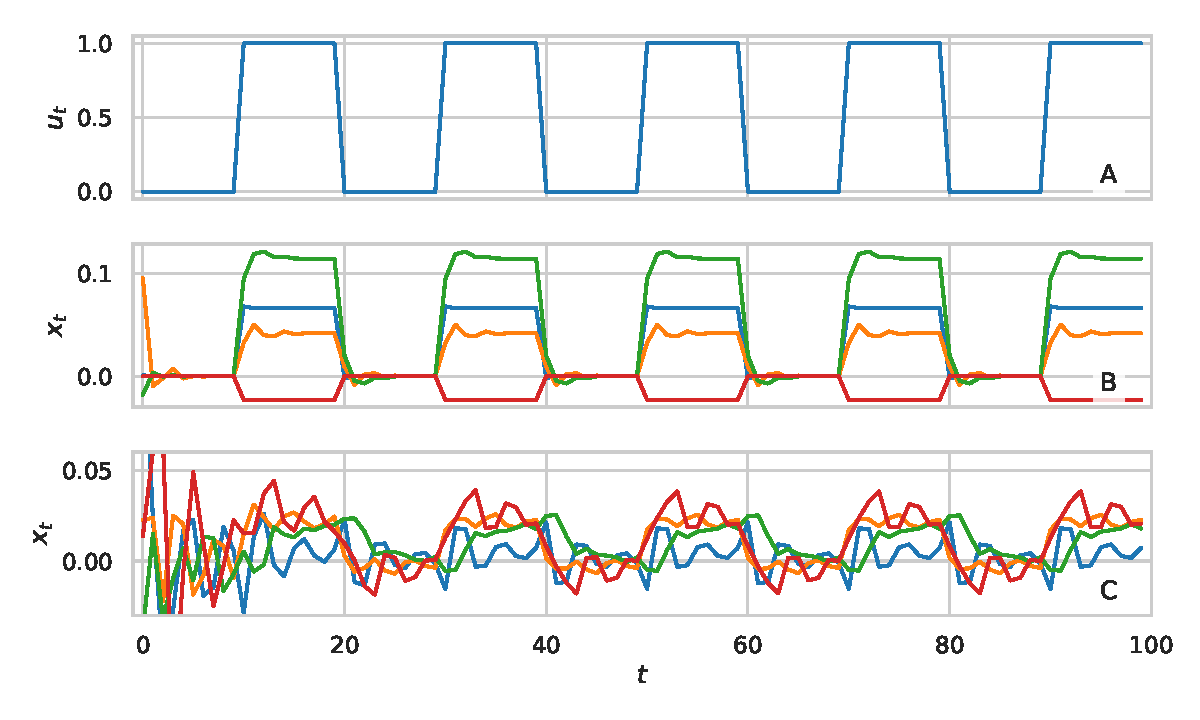
\includegraphics[width=\linewidth]{esn_states_input.pdf}
  \caption{Reaction of the internal state of the ESN to external input $u(t)$
  (step function in graph A).
  A large $\kappa$ leads to the input dominating the internal state, while a
  smaller $\kappa$ enables it to memorize previous inputs.}
  \label{fig:esn_states_input}
\end{figure}

Both $\rho$ and $\kappa$ must be chosen with respect to the task at hand.  The
last hyper-parameter of the ESN is the sparsity of the reservoir matrix
$\wmatr{}$. It only affects ESN memory for values well above 95\%
[\cite{farkavs2016}], but it can significantly reduce computational complexity
for large reservoir sizes.  The specific choice of these parameters can be made
with a hyper-parameter optimizer, as described in
Sec.~\ref{sec:hyper_parameter_optimization}.


\subsection{Short-term Memory \& Reservoir Non-linearity}%
\label{sub:short_term_memory}

Short-term memory describes the dynamic memory of an internal ESN (or more
generally RNN) state, which should not be confused with the memory of a network
that is brought about by weight adaptions (e.g. through gradient descent),
which is called long-term memory.  We have already convinced ourselves that the
internal state acts as a memory of the previous inputs, as depicted in
Fig.~\ref{fig:esn_states_noinput}.  This memory could be almost arbitrarily
long if it were not for the problem of vanishing gradients of very deep
networks, which bounds the length of a practically learnable sequence to a
number of data points in the order of ten.  As already discussed, ESNs avoid
the vanishing gradient problem altogether by not calculating recurrent
gradients at all. Without this problem, how much can an ESN remember?  It was
shown by [\cite{jaeger2002}] that for linear recurrent weights (where the
activation function is the identity) the \emph{memory capacity} (MC) is equal
to the size of the ESN state:
\begin{equation}
  \text{MC} = N_{units} \text{ .}
\end{equation}

The memory capacity is defined as the number of inputs that a perfectly trained
output matrix $\wmatr{out}$ can extract from an ESN state which was created by
feeding it a random sequence.  A random sequence in this context means a series
of numbers that were drawn from a uniform distribution. How to practically measure
MC is shown in Sec.~\ref{sec:short_term_memory}. Essentially the value of the MC
give a measure of how many input steps the ESN can encode in its internal state.

For the case of a non-linear activation function in the recurrency of the ESN
the MC has an upper bound:
\begin{equation}
  \text{MC} < N_{units} \text{ .}
\end{equation}

Intuitively one might think that a larger MC will
automatically lead to a better performing prediction. However, there is a
second requirement that needs to be fulfilled in order to predict chaotic
systems well: The degree of non-linearity (essentially expressed by the
spectral radius) of the reservoir must be appropriate for the task.
A network with the hyperbolic tangent as an activation function and 
a spectral radius close to or smaller than one acts mostly in the
linear regime of the tanh. This means that the dynamics of the internal state
are governed by an approximately linear expansion and in turn makes it very
hard for the (also linear) output layer to produce a chaotic prediction.
The obvious solution is to increase the spectral radius to values greater than
one, but it turns out that there is a tradeoff between MC and the non-linearity
of the ESN reservoir. Increasing the spectral radius above one degrades the
memory of the ESN (Sec.~\ref{sec:short_term_memory}), but makes it possible
to predict chaotic systems (Sec.~\ref{sec:res_mackey_glass_system}).
A potential solution to this problem lies in separating the memory of the ESN
from is linear transformation. This was attempted with an extension of the ESN
to R$^2$SP (random static projections) by [\cite{butcher2013}], but its treatment
is out of the scope of this work.


\subsection{ESN Training}
\label{sub:esn_training}

To train an ESN any of the previously introduced methods for training RNNs can
be used. The fact that only the last layer is trained makes an additional, much
faster least squared method possible.  In the case of a linear output layer,
the predictions of the network can be written as
\begin{equation}
  \vt{y} = \wmatr{out} \vt{x},
  \label{eq:esn_lin_out}
\end{equation}
where $\vt{x}$ can generally either be the internal state or the internal state
concatenated with the corresponding input $\vt{u}$.  By collecting a number of
states (and inputs) that are created with the untrained network, we can rewrite
Eq.~\ref{eq:esn_lin_out} into Eq.~\ref{eq:esn_lin_out_concat} with concatenated
states $\matr{X}$ and desired outputs $\matr{D}$.
\begin{align}
  \matr{X} &:= (\vec{x}_1, ..., \vec{x}_T) \\
  \matr{D} &:= (\vec{d}_1, ..., \vec{d}_T) \\
  \matr{D} &= \wmatr{out} \matr{X} \label{eq:esn_lin_out_concat}
\end{align}

To find the optimal weights $\wmatr{out}$ we have to solve the overdetermined
system in Eq.~\ref{eq:esn_lin_out_concat}, which can be done for example via
the pseudo-inverse method.  It even gets by without introducing an
additional hyper-parameter by utilizing the Moore-Penrose pseudo-inverse
$\matr{X}^+$:

\begin{align}
  \wmatr{out} &= \matr{D}\matr{X}^+ \\
  \matr{X}^+  &= (\matr{X}^T\matr{X})^{-1} \matr{X}^T
\end{align}



Another method is called \emph{Tikhonov Regularization}, which, outside
geophysical contexts, is more frequently called \emph{ridge
regression}~[\cite{MontgomeryRegression}]:
\begin{equation}
  \label{eq:tikhonov}
  \wmatr{out} = \matr{D} \XT (\matr{X} \XT - \beta \matr{I})^{-1}
\end{equation}
The regularization coefficient $\beta$ is introduced to reduce the risk of
overfitting the output weights, which will quickly lead to diverging
predictions when feeding the output of the ESN back into the input.
Effectively $\beta$ becomes another hyper-parameter, which has to be tuned in
order to obtain good results.  A derivation of Tikhonov Regularization can be
found in the Appendix~\ref{sec:tikhonov_regularization}.  
